\documentclass[usenames,dvipsnames]{beamer}
%\documentclass[handout]{beamer}

\usetheme{Warsaw}

\usepackage{epstopdf}
\usepackage{graphicx}
\usepackage{subfigure}
\usepackage{comment}
\usepackage{array}


% Predicate language syntax highlighting
\usepackage{listings}
\definecolor{keywordblue}{RGB}{20,105,176}
\lstdefinelanguage{Hoppy}{
    morekeywords=[1]{all,function,as,returning,in,using},
    morekeywords=[2]{this},
    morekeywords=[3]{int,float},
    morekeywords=[4]{Neighbours,abs,mean,max,min,sum,len},
    sensitive=true,
}
\lstset{
    language=Hoppy,
    keywordstyle=[1]\color{keywordblue},
    keywordstyle=[2]\color{OliveGreen},
    keywordstyle=[3]\color{YellowOrange},
    keywordstyle=[4]\color{Purple},
    basicstyle=\ttfamily,
    columns=fullflexible,
}

\lstdefinelanguage{Dragon}{
    morekeywords=[1]{IPUSH,IPOP,IFETCH,ISTORE,IADD,ISUB,IMUL,IDIV1,IDIV2,IINC,IDEC,IEQ,INEQ,ILT,ILEQ,IGT,IGEQ,IABS,IVAR,ICASTF},
    morekeywords=[2]{FPUSH,FPOP,FFETCH,FSTORE,FADD,FSUB,FMUL,FDIV1,FDIV2,FEQ,FNEQ,FLT,FLEQ,FGT,FGEQ,FABS,FVAR,FCASTI},
    morekeywords=[3]{AFETCH,ALEN,ASUM,AMEAN,AMAX,AMIN},
    morekeywords=[4]{HALT,CALL,JMP,JZ,JNZ},
    morekeywords=[5]{VIINC,VIDEC,VIFAFC,THISC},
    morekeywords=[6]{AND,OR,XOR,EQUIVALENT,IMPLIES,NOT},
    morecomment=[l]{//},
    sensitive=true,
}
\lstset{
    language=Dragon,
    keywordstyle=[1]\color{Cyan},
    keywordstyle=[2]\color{WildStrawberry},
    keywordstyle=[3]\color{YellowOrange},
    keywordstyle=[4]\color{Violet},
    keywordstyle=[5]\color{ForestGreen},
    keywordstyle=[6]\color{BurntOrange},
    basicstyle=\ttfamily,
    columns=fullflexible,
}

\setbeamertemplate{blocks}[framed]
\setbeamercolor{block title}{use={frametitle},fg=frametitle.fg,bg=frametitle.bg}

\newcommand{\subtitleframe}[1]{\begin{frame}\begin{block}{\centering\Large \vspace{1em} #1 \vspace{1em}}\end{block}\end{frame}}

%\usepackage{pgfpages}
%\pgfpagesuselayout{4 on 1}[a4paper,landscape,border shrink=3mm]

\title{Towards Practical Debugging of Wireless Sensor Networks}
\author[M.~Bradbury, T.~Law, I.~Leon, D.~Robertson, A.~Shah, J.~Yarnall]{Matthew Bradbury\newline
Tim Law\newline
Ivan Leong\newline
Dan Robertson\newline
Amit Shah\newline
Joe Yarnall}
\institute{CS407: Fourth Year Project}
\date{10--11AM Tuesday 7th May 2013}

\begin{document}

\begin{frame}
\titlepage
\end{frame}

\subtitleframe{Introduction}

%Matt
\begin{frame}{What is a Wireless Sensor Network}
A wireless sensor network (WSN) is a collection of computing devices called motes, they have:
	\begin{itemize}
		\item a short range wireless radio
		\item an array of sensors such as light, heat and humidity
		\item a simple low powered CPU
		\item a battery with limited power supply
	\end{itemize}
Motes communicate with each other to form a WSN.
WSNs perform data gathering tasks such as environment monitoring.
\end{frame}

%Matt
\begin{frame}{The Problem of Debugging Distributed Systems}
	\begin{itemize}
		\item Multiple tasks running simultaneously leads to non--deterministic interactions
		\item Traditional debugging tools are unsuited
		\item Timing and synchronisation issues
	\end{itemize}
\end{frame}

%Matt
\begin{frame}{Complications to the Problem}
	\begin{itemize}
		\item Motes are energy constrained
		\item Sending messages is the most expensive task
		\item Receiving messages is the next most expensive task \cite{Shnayder04}
		\item Motes have low computing power and a small memory
		\item WSNs deployed in hard to reach areas --- physical access after deployment is difficult \cite{herbert2007adaptive}
	\end{itemize}
\end{frame}

%Matt
\begin{frame}{Related Work}
	\begin{itemize}
		\item Global Predicate Detection \cite{553309}
		\item H--SEND \cite{herbert2007adaptive}
		\item NodeMD \cite{NodeMD}
		\item TinyOS \cite{tinyos}, Contiki
	\end{itemize}
\end{frame}

%Matt
\begin{frame}{Project Aims}
	\begin{itemize}
		\item Develop tools to aid in debugging distributed programs running on WSNs.
		\item Implement libraries that check predicates, with a focus on correctly evaluating these predicates.
		\item Investigate if there are places in the network where evaluation is more efficient.
		\item Visualise some of the state of the network, as part of a tool to inform system users what state the network is in.
	\end{itemize}
\end{frame}

%Matt
\begin{frame}{Project Management}
	\begin{itemize}
		\item Matthew --- Group Leader
		\item Amit --- Technical Manager
		\item Everyone was involved with development and research
		\item Bitbucket.org Git repository
	\end{itemize}
\end{frame}

%Joe
\subtitleframe{Implemented Libraries}

%Joe
\begin{frame}{Implemented Libraries --- Containers}
	\begin{itemize}
		\item Linked List
			\begin{itemize}
				\item Our's: Standard linked list
				\item Contiki's: Intrusive linked list
			\end{itemize}
		\item Array List
		\item Unique Array
		\item Map
	\end{itemize}
\vspace{1em}
Benefits:
	\begin{itemize}
		\item Abstraction
		\item Reduced code duplication
		\item Simplified memory management
	\end{itemize}
\end{frame}

%Joe
\begin{frame}{Implemented Libraries --- N--Hop Request}
	\begin{itemize}
		\item Used by predicate evaluation
		\item Floods request N--Hops away from sink
		\item Asks for motes current state
		\item Returned along the chain created by the flooding stage
	\end{itemize}

\begin{figure}[H]
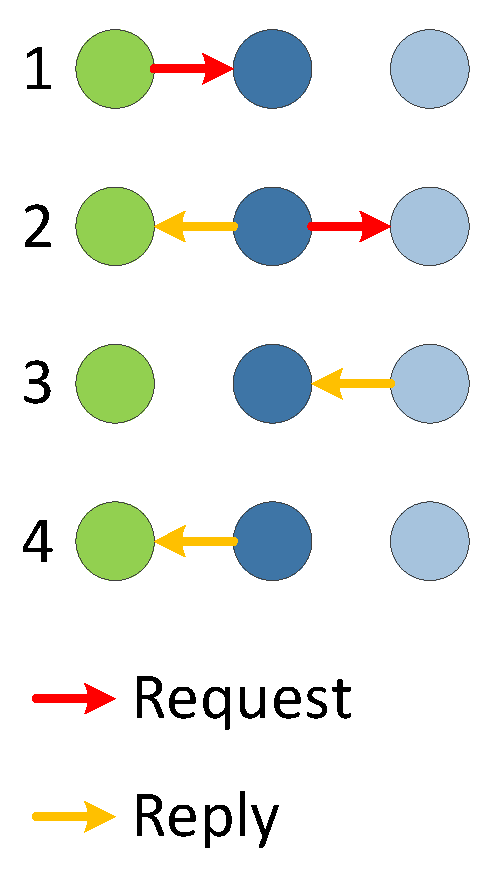
\includegraphics[scale=0.3]{../Report/Diagrams/n-hop-flood-req-reply.eps}\hspace{1em}
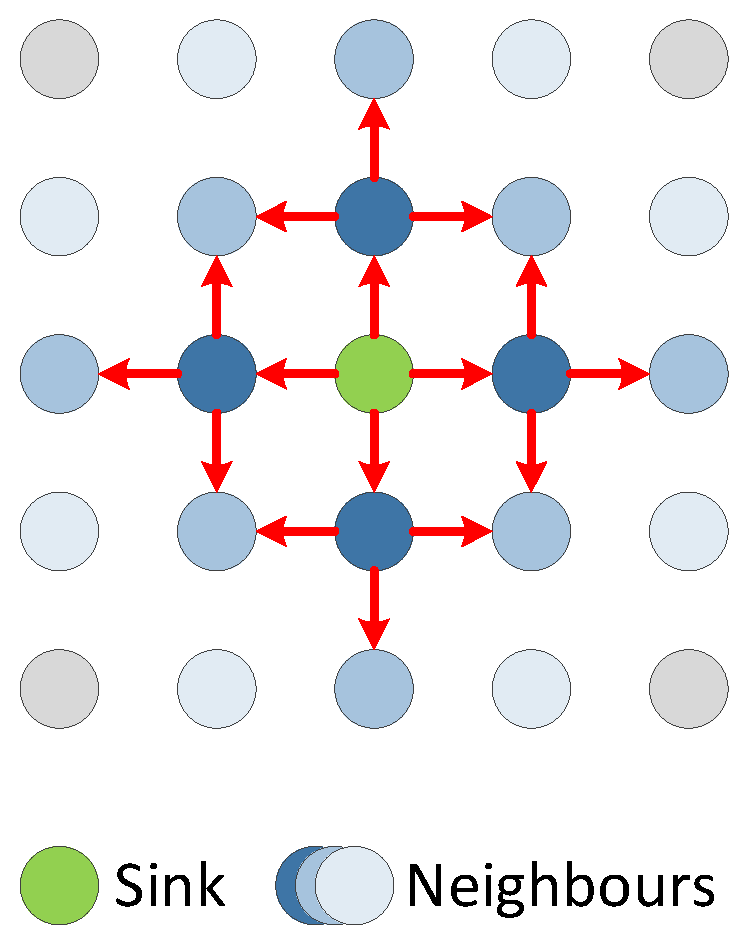
\includegraphics[scale=0.3]{../Report/Diagrams/2-hop-flooding.eps}
\end{figure}
\end{frame}

%Joe
\begin{frame}{Implemented Libraries --- N--Hop Flood}
	\begin{itemize}
		\item Floods a given packet N hops
		\item Surprised that Contiki did not provide this as a library
			\begin{itemize}
				\item Had to implement ourselves using TTLs in packet headers
			\end{itemize}
	\end{itemize}
\end{frame}

%Joe
\begin{frame}{Implemented Libraries --- Event Update}
	\begin{itemize}
		\item Used by predicate evaluation
		\item Periodically checks if node's data has changed
		\item If it has floods the new data the required number of hops
	\end{itemize}
\vspace{1em}
Depends On:
	\begin{itemize}
		\item N--Hop Flood
	\end{itemize}
\end{frame}

%Joe
\begin{frame}{Implemented Libraries --- Multi--Packet Unicast}
	\begin{itemize}
		\item Contiki packet size: 128 bytes
		\item This is too small for some of our data
		\item Alternative APIs Contiki implements are convoluted
			\begin{itemize}
				\item Targeted towards sending file chunks
			\end{itemize}
		\item We split packet up, send pieces and then reassemble
	\end{itemize}
\end{frame}

%Joe
\begin{frame}{Implemented Libraries --- Tree Aggregation}
	\begin{enumerate}
		\item Leaf node generates data, forwards to parent
		\item Parent waits for a period, aggregating received data
		\item The node adds its own data to the aggregate
		\item The node then forwards the message to its parent
		\item Repeat until the aggregated message reaches the base station
	\end{enumerate}
\vspace{1em}
Again surprised that Contiki didn't have an implementation\newline

Depends On:
	\begin{itemize}
		\item Multi--Packet
	\end{itemize}
\end{frame}

%Joe
\begin{frame}{Implemented Libraries --- Neighbour Detection}
	\begin{itemize}
		\item To debug a WSN we need to know the network topology
		\item Uses Tree Aggregation to send neighbours to sink
	\end{itemize}

\begin{figure}[H]
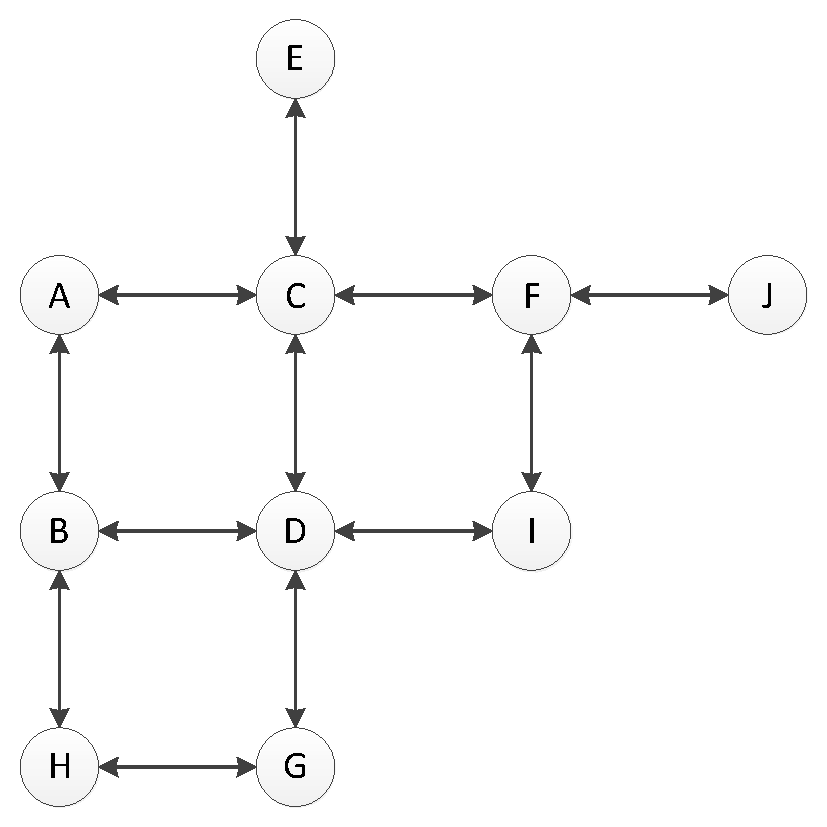
\includegraphics[scale=0.35]{../Report/Diagrams/neighbour-network.eps}\hspace{1em}
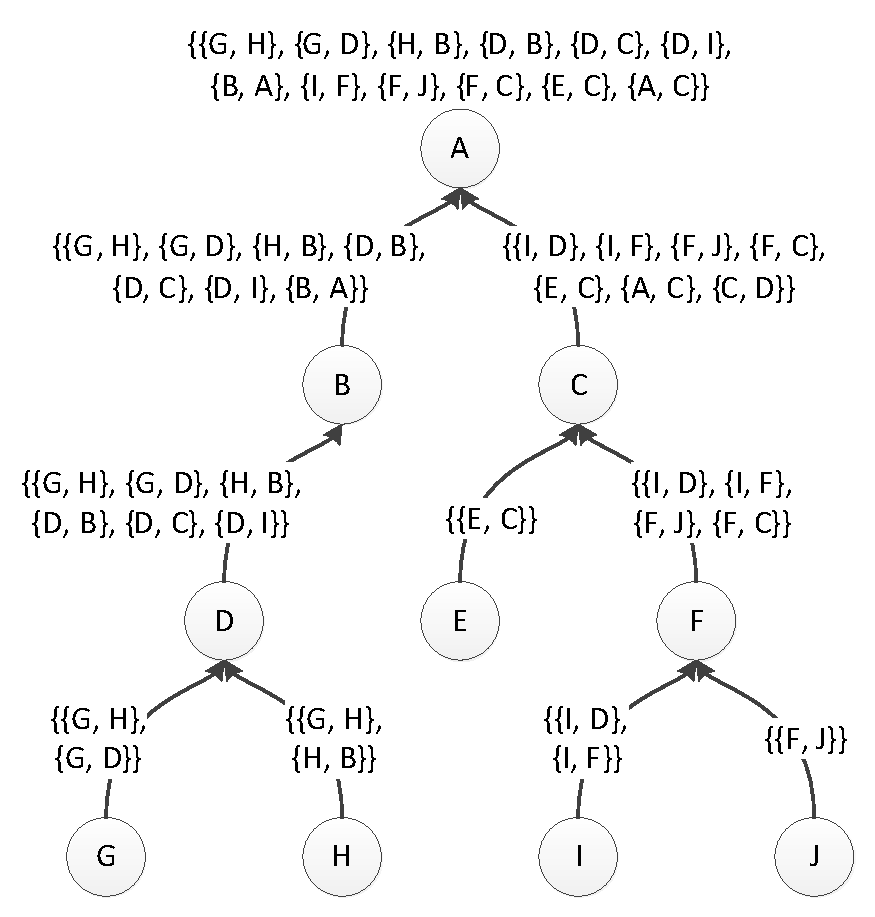
\includegraphics[scale=0.35]{../Report/Diagrams/neighbour-tree-structure.eps}
\end{figure}
\end{frame}

%Matt
\subtitleframe{Predicate Evaluation}

%Matt
\begin{frame}{Predicate Evaluation}
	\begin{enumerate}
		\item Disseminate predicate to network
		\item Evaluate predicate
		\item Return response to base station
	\end{enumerate}
\vspace{1em}

Consider:
	\begin{itemize}
		\item Where to evaluate: Local vs. Global
		\item When to propagate mote data: Periodic vs. Event
		\item How to respond to a failure or success
	\end{itemize}
\end{frame}

%Matt
\begin{frame}[allowframebreaks]{Predicate Evaluation --- Libraries}
\begin{table}[H]
\centering
\begin{tabular}{| l | p{4.2cm} | p{4.2cm} |}
\hline
~ & Periodic & Event\\
\hline
Local & PELP
	\begin{itemize}
		\item Evaluated in--network
		\item Data is requested when needed to evaluate predicate
		\item Previous round's data is forgotten after a round completes
	\end{itemize}
 & PELE
	\begin{itemize}
		\item Evaluated in--network
		\item Data is sent by data sources, when it changes
		\item Data is never forgotten, simply updated
	\end{itemize}\\
\hline
\end{tabular}
\end{table}

\begin{table}[H]
\centering
\begin{tabular}{| l | p{4.2cm} | p{4.2cm} |}
\hline
~ & Periodic & Event\\
\hline
Global & PEGP
	\begin{itemize}
		\item Similar to PELP, except data is aggregated to the base station
	\end{itemize}
 & PEGE
	\begin{itemize}
		\item Similar to PELE, except data is aggregated to the base station
	\end{itemize}\\
\hline
\end{tabular}
\end{table}
\end{frame}


%Matt
\begin{frame}{Predicate Evaluation --- Libraries Used}
\begin{table}[H]
\centering
\begin{tabular}{| l | p{4.2cm} | p{4.2cm} |}
\hline
~ & Periodic & Event\\
\hline
Local & PELP
	\begin{itemize}
		\item N--Hop Request
	\end{itemize}
 & PELE
	\begin{itemize}
		\item Event Update
			\begin{itemize}
				\item N--Hop Flood
			\end{itemize}
	\end{itemize}\\
\hline
Global & PEGP
	\begin{itemize}
		\item Neighbour Detect
		\item Tree Aggregation
	\end{itemize}
 & PEGE
	\begin{itemize}
		\item Neighbour Detect
		\item Tree Aggregation
	\end{itemize}\\
\hline
\end{tabular}
\end{table}
\end{frame}

%Matt
\begin{frame}{Predicate Evaluation --- Response}
\begin{columns}[t]
	\begin{column}[T]{5cm}
		Failure
		\begin{itemize}
			\item Only predicate failures are reported to the base station
			\item Cannot say much about the network state, either:
				\begin{itemize}
					\item we have not been informed of a failure
					\item we have been informed
				\end{itemize}
			\item We chose this one due to the reduced traffic
		\end{itemize}
	\end{column}
	\begin{column}[T]{5cm}
		Failure and Success
		\begin{itemize}
			\item Both failures and successes are reported
			\item Supports detecting the network is in the following states:
				\begin{itemize}
					\item Unknown
					\item Failed
					\item Succeeded
					\item Failed and then later succeeded
				\end{itemize}
			\item Uses more energy
		\end{itemize}
	\end{column}
	\end{columns}
	\vspace{1em}

	Note: Global PE may as well take advantage of "Failure and Success" messages, as the target of them is the node the predicates are evaluated on
\end{frame}

%Matt
\begin{frame}{Predicate Evaluation --- Evaluation}
\begin{itemize}
	\item Implemented a virtual machine in C to evaluate predicates on the nodes
		\begin{itemize}
			\item Optimised for low memory environment
			\item Opcodes for high--level operations to reduce program size
		\end{itemize}
	\vspace{1em}
	\item Implemented a DSL with a JavaCC parser and a Java compiler and assembler
		\begin{itemize}
			\item Functional language
			\item Expects a boolean output
		\end{itemize}
\end{itemize}
\end{frame}


%Matt
\begin{frame}[fragile]{Predicate Evaluation --- DSL}
\begin{align*}
&				\forall n \in \text{Nodes} \cdot \\
& \hspace{2em}		\forall n' \in \text{Neighbours}(n, 2) \cdot \\
& \hspace{4em}				\text{slot}(n) \neq \text{slot}(n')
\end{align*}

\begin{center}
\begin{minipage}{0.75\textwidth}
\begin{lstlisting}[language=Hoppy]
[all]
function 1 as slot returning int in
    using Neighbours(2) as twohopn in
        @(x : twohopn ~
            slot(x) != slot(this)
        )
\end{lstlisting}
\end{minipage}
\end{center}

\end{frame}

%Matt
\begin{frame}[fragile]{Predicate Evaluation --- DSL}
\begin{align*}
&				\forall n \in \text{Nodes} \cdot \\
& \hspace{2em}		\forall n' \in \text{Neighbours}(n, 1) \cup \{n\} \cdot \\
& \hspace{4em}			\forall n'' \in \text{Neighbours}(n, 1) \cup \{n\} \cdot \\
& \hspace{6em}				\text{addr}(n') \not= \text{addr}(n'') \\
& \hspace{8em}					\implies \text{slot}(n') \neq \text{slot}(n'')
\end{align*}

\begin{center}
\begin{minipage}{0.75\textwidth}
\begin{lstlisting}[language=Hoppy]
[all]
function 0 as addr returning int in
function 1 as slot returning int in
    using Neighbours(1) as ohn in
        @(a : ohn ~
            @(b : ohn ~ addr(a) != addr(b)
                => slot(a) != slot(b))
            & slot(a) != slot(this)
        )
\end{lstlisting}
\end{minipage}
\end{center}
\end{frame}

%Matt
\begin{frame}[fragile]{Predicate Evaluation --- DSL}
\begin{columns}[t]
	\begin{column}[T]{3.1cm}
\begin{lstlisting}[language=Dragon]
//TARGETING all
//FUNC 0 AS addr
//FUNC 1 AS slot
//STORING 1 IN ohn
IVAR 1
IPUSH 1
IPUSH 0
ISTORE 1
start1: ALEN 255
INEQ
JZ end1
IVAR 2
IPUSH 1
IPUSH 0
ISTORE 2
start2: ALEN 255
\end{lstlisting}
	\end{column}
	\begin{column}[T]{2.6cm}
\begin{lstlisting}[language=Dragon]
INEQ
JZ end2
//addr(a[*1])
VIFAFC 1 255 0
//addr(b[*2])
VIFAFC 2 255 0
INEQ
//slot(a[*1])
VIFAFC 1 255 1
//slot(b[*2])
VIFAFC 2 255 1
INEQ
IMPLIES
AND
VIINC 2
JMP start2
\end{lstlisting}
	\end{column}
\begin{column}[T]{3.4cm}
\begin{lstlisting}[language=Dragon]
//slot(a[*1])
end2: VIFAFC 1 255 1
//slot(this)
THISC 1
INEQ
AND
AND
VIINC 1
JMP start1
end1: HALT
//VD 1 = 255
\end{lstlisting}
	\end{column}
	\end{columns}

\end{frame}


%Matt
\subtitleframe{Results}

\begin{frame}{Results Methodology}
\begin{itemize}
	\item Run and measure energy usage of TDMA algorithm
	\item Measure energy cost of predicate evaluation algorithm
		\begin{itemize}
			\item Checking for slot collisions
			\item Vary predicate distance (1--hop and 2--hop)
			\item Vary predicate evaluation algorithm
		\end{itemize}
	\item Network was laid out as a grid
	\item N, S, E, W communication possible
	\item 5 minutes setup time for PE, start TDMA
	\item 35 minutes total runtime
\end{itemize}
\end{frame}

\begin{frame}{Results when period=4.0 minutes using a 1--hop predicate}
\begin{figure}[H]
\centering
\subfigure[Rx]{%
	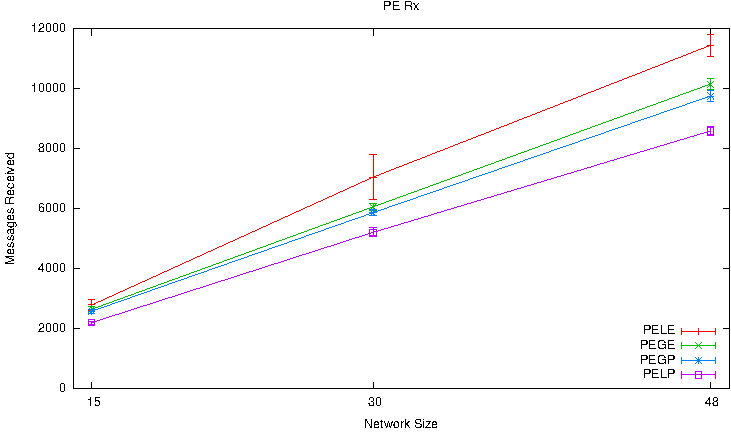
\includegraphics[width=0.45\linewidth]{../Results/Graphs/4.0/1HOP/messagesPE/rx/graph.pdf}
}
\subfigure[Tx]{%
	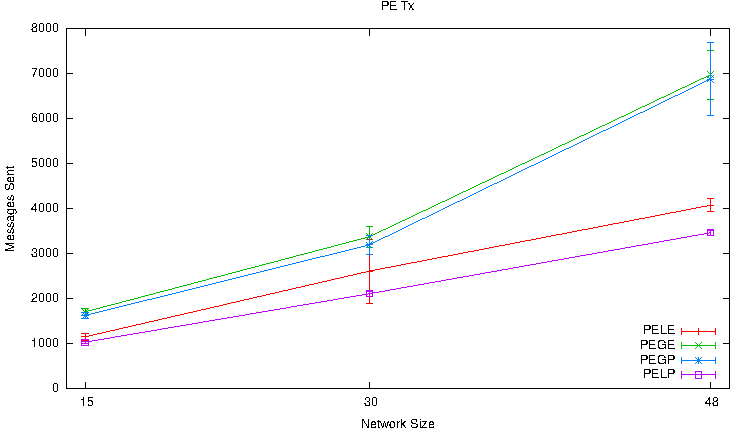
\includegraphics[width=0.45\linewidth]{../Results/Graphs/4.0/1HOP/messagesPE/tx/graph.pdf}
}

\subfigure[Percentage of  predicates correctly evaluated]{%
	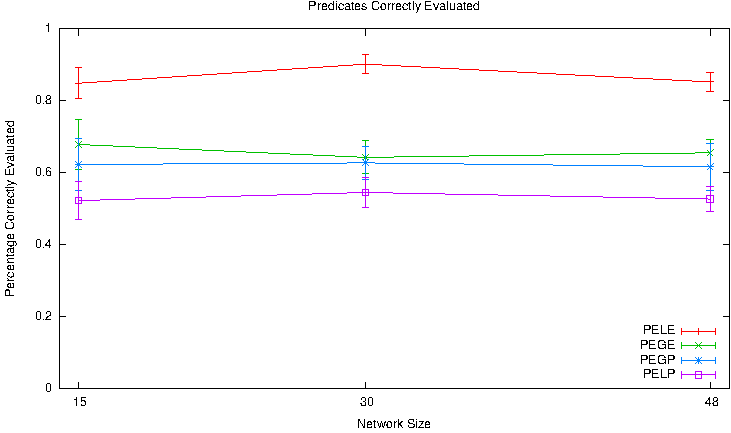
\includegraphics[width=0.45\linewidth]{../Results/Graphs/4.0/1HOP/pcCorrectlyEvaluated/graph.pdf}
}
\subfigure[Percentage of responses received]{%
	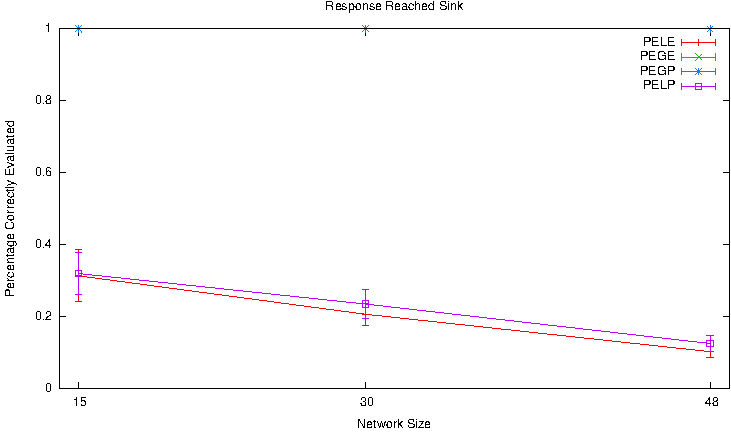
\includegraphics[width=0.45\linewidth]{../Results/Graphs/4.0/1HOP/pcResponsesReachedSink/graph.pdf}
}
\end{figure}
\end{frame}

\begin{frame}{Results when period=4.0 minutes using a 2--hop predicate}
\begin{figure}[H]
\centering
\subfigure[Rx]{%
	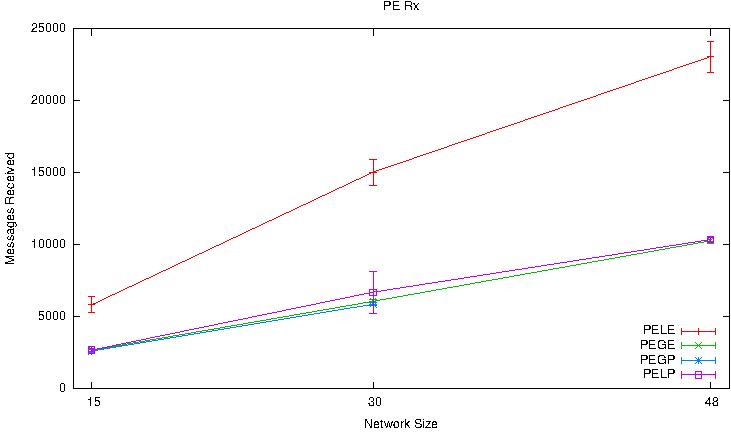
\includegraphics[width=0.45\linewidth]{../Results/Graphs/4.0/2HOP/messagesPE/rx/graph.pdf}
}
\subfigure[Tx]{%
	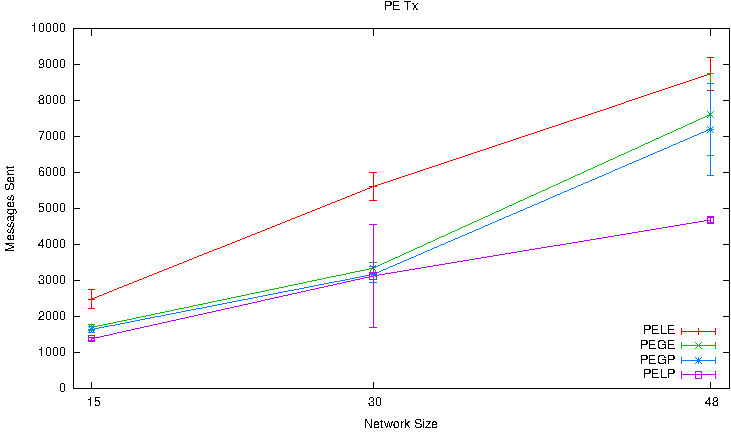
\includegraphics[width=0.45\linewidth]{../Results/Graphs/4.0/2HOP/messagesPE/tx/graph.pdf}
}

\subfigure[Percentage of  predicates correctly evaluated]{%
	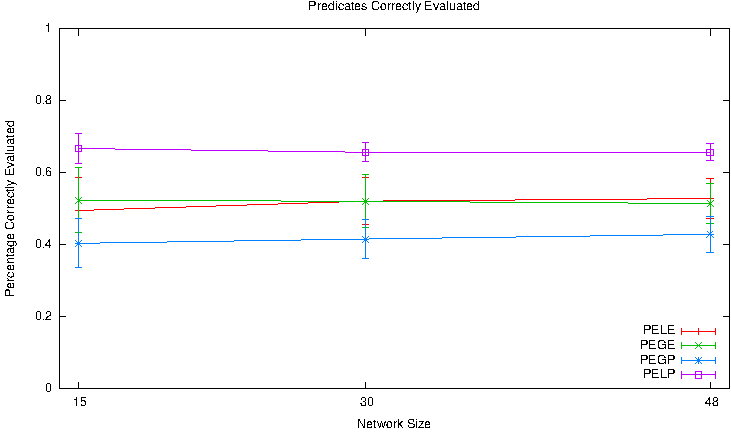
\includegraphics[width=0.45\linewidth]{../Results/Graphs/4.0/2HOP/pcCorrectlyEvaluated/graph.pdf}
}
\subfigure[Percentage of responses received]{%
	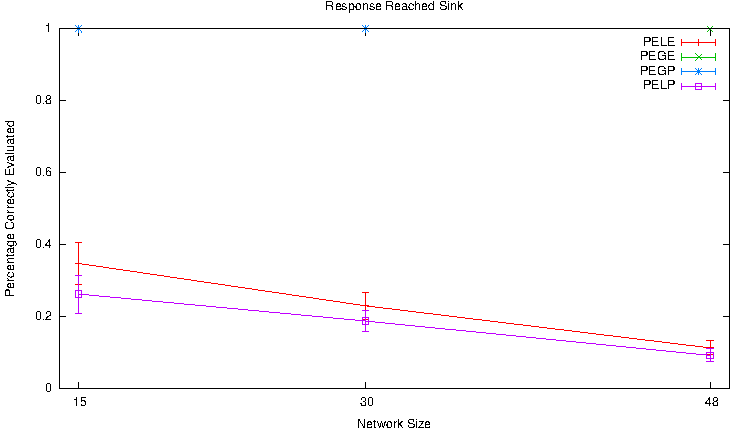
\includegraphics[width=0.45\linewidth]{../Results/Graphs/4.0/2HOP/pcResponsesReachedSink/graph.pdf}
}
\end{figure}
\end{frame}


\subtitleframe{Demo}

\begin{frame}{Visualisation Tool and Network Interface}
Features:
\begin{itemize}
	\item Creating and compiling predicates to monitor
	\item Deploying predicates to the WSN
	\item Recording history of evaluation results
	\item Use of \texttt{serialdump-linux} to interface with sink mote
\end{itemize}
\vspace{1em}

Views:
\begin{itemize}
	\item Predicate view
	\item Network view
\end{itemize}
\end{frame}


\subtitleframe{Conclusions}

\begin{frame}{Future Work}
	\begin{itemize}
		\item Improve memory management
		\item Improve C containers developed
		\item Stateful predicates
		\item Handle mote mobility
		\item Improve failure response message deliver ratio
	\end{itemize}
\end{frame}

\begin{frame}{Summary}
Developed:
	\begin{itemize}
		\item Libraries for use in Contiki (Container and Network)
		\item Predicate Evaluation Libraries (Global and Local)
		\item GUI tool to interface with network
	\end{itemize}
\vspace{1em}

Found:
	\begin{itemize}
		\item In--network, event--based evaluation suitable for ``small'' predicates
		\item Global, periodic evaluation more suitable for ``large'' predicates
	\end{itemize}
\end{frame}

\begin{frame}[allowframebreaks]{References}
	\bibliographystyle{apalike}
	\bibliography{../References/references,../References/BradburyCS310}
\end{frame}

\begin{frame}{The End}
Any Questions?
\end{frame}

\end{document}